\chapter{Metodología}

En este capítulo describimos en profundidad todos los pasos seguidos en los métodos empleados en el trabajo y su justificación. Posteriormente, se aplicarán en la experimentación.

\section{Análisis de los recursos disponibles}

Para la realización de este trabajo debemos considerar los recursos hardware disponibles para la inferencia de los modelos pero sobre todo para el entrenamiento de los modelos.

\begin{enumerate}
	\item \textbf{Hardware en entrenamiento}. Para el desarrollo de toda la experimentación, entrenamiento de los modelos y validación nos valdremos de los recursos que gratuitamente ofrece Kaggle, una plataforma de ciencia de datos propiedad de Google. 
	
	El recurso más importante que ofrece Kaggle y razón de su uso es que nos permite el uso de su gráfica NVIDIA Tesla P100 por 30 horas semanales. Con ella, podemos entrenar los modelos y hacer una inferencia rápida para validación en tiempo razonable.
	
	Por nosotros mismos sólo disponíamos de un ordenador personal que aunque con mejor disponibilidad de memoria en disco $\approx 2\ TB$ que la ofrecida por Kaggle $\approx 100\ GB$, nuestra gráfica NVIDIA GeForce RTX 2060 tiene inmensamente menores prestaciones que la ofrecida en Kaggle. A continuación, mostramos una gráfica de rendimiento sobre las características de ambos dispositivos para cuantificar este hecho.
	
	\begin{figure}[H]
		\centering
		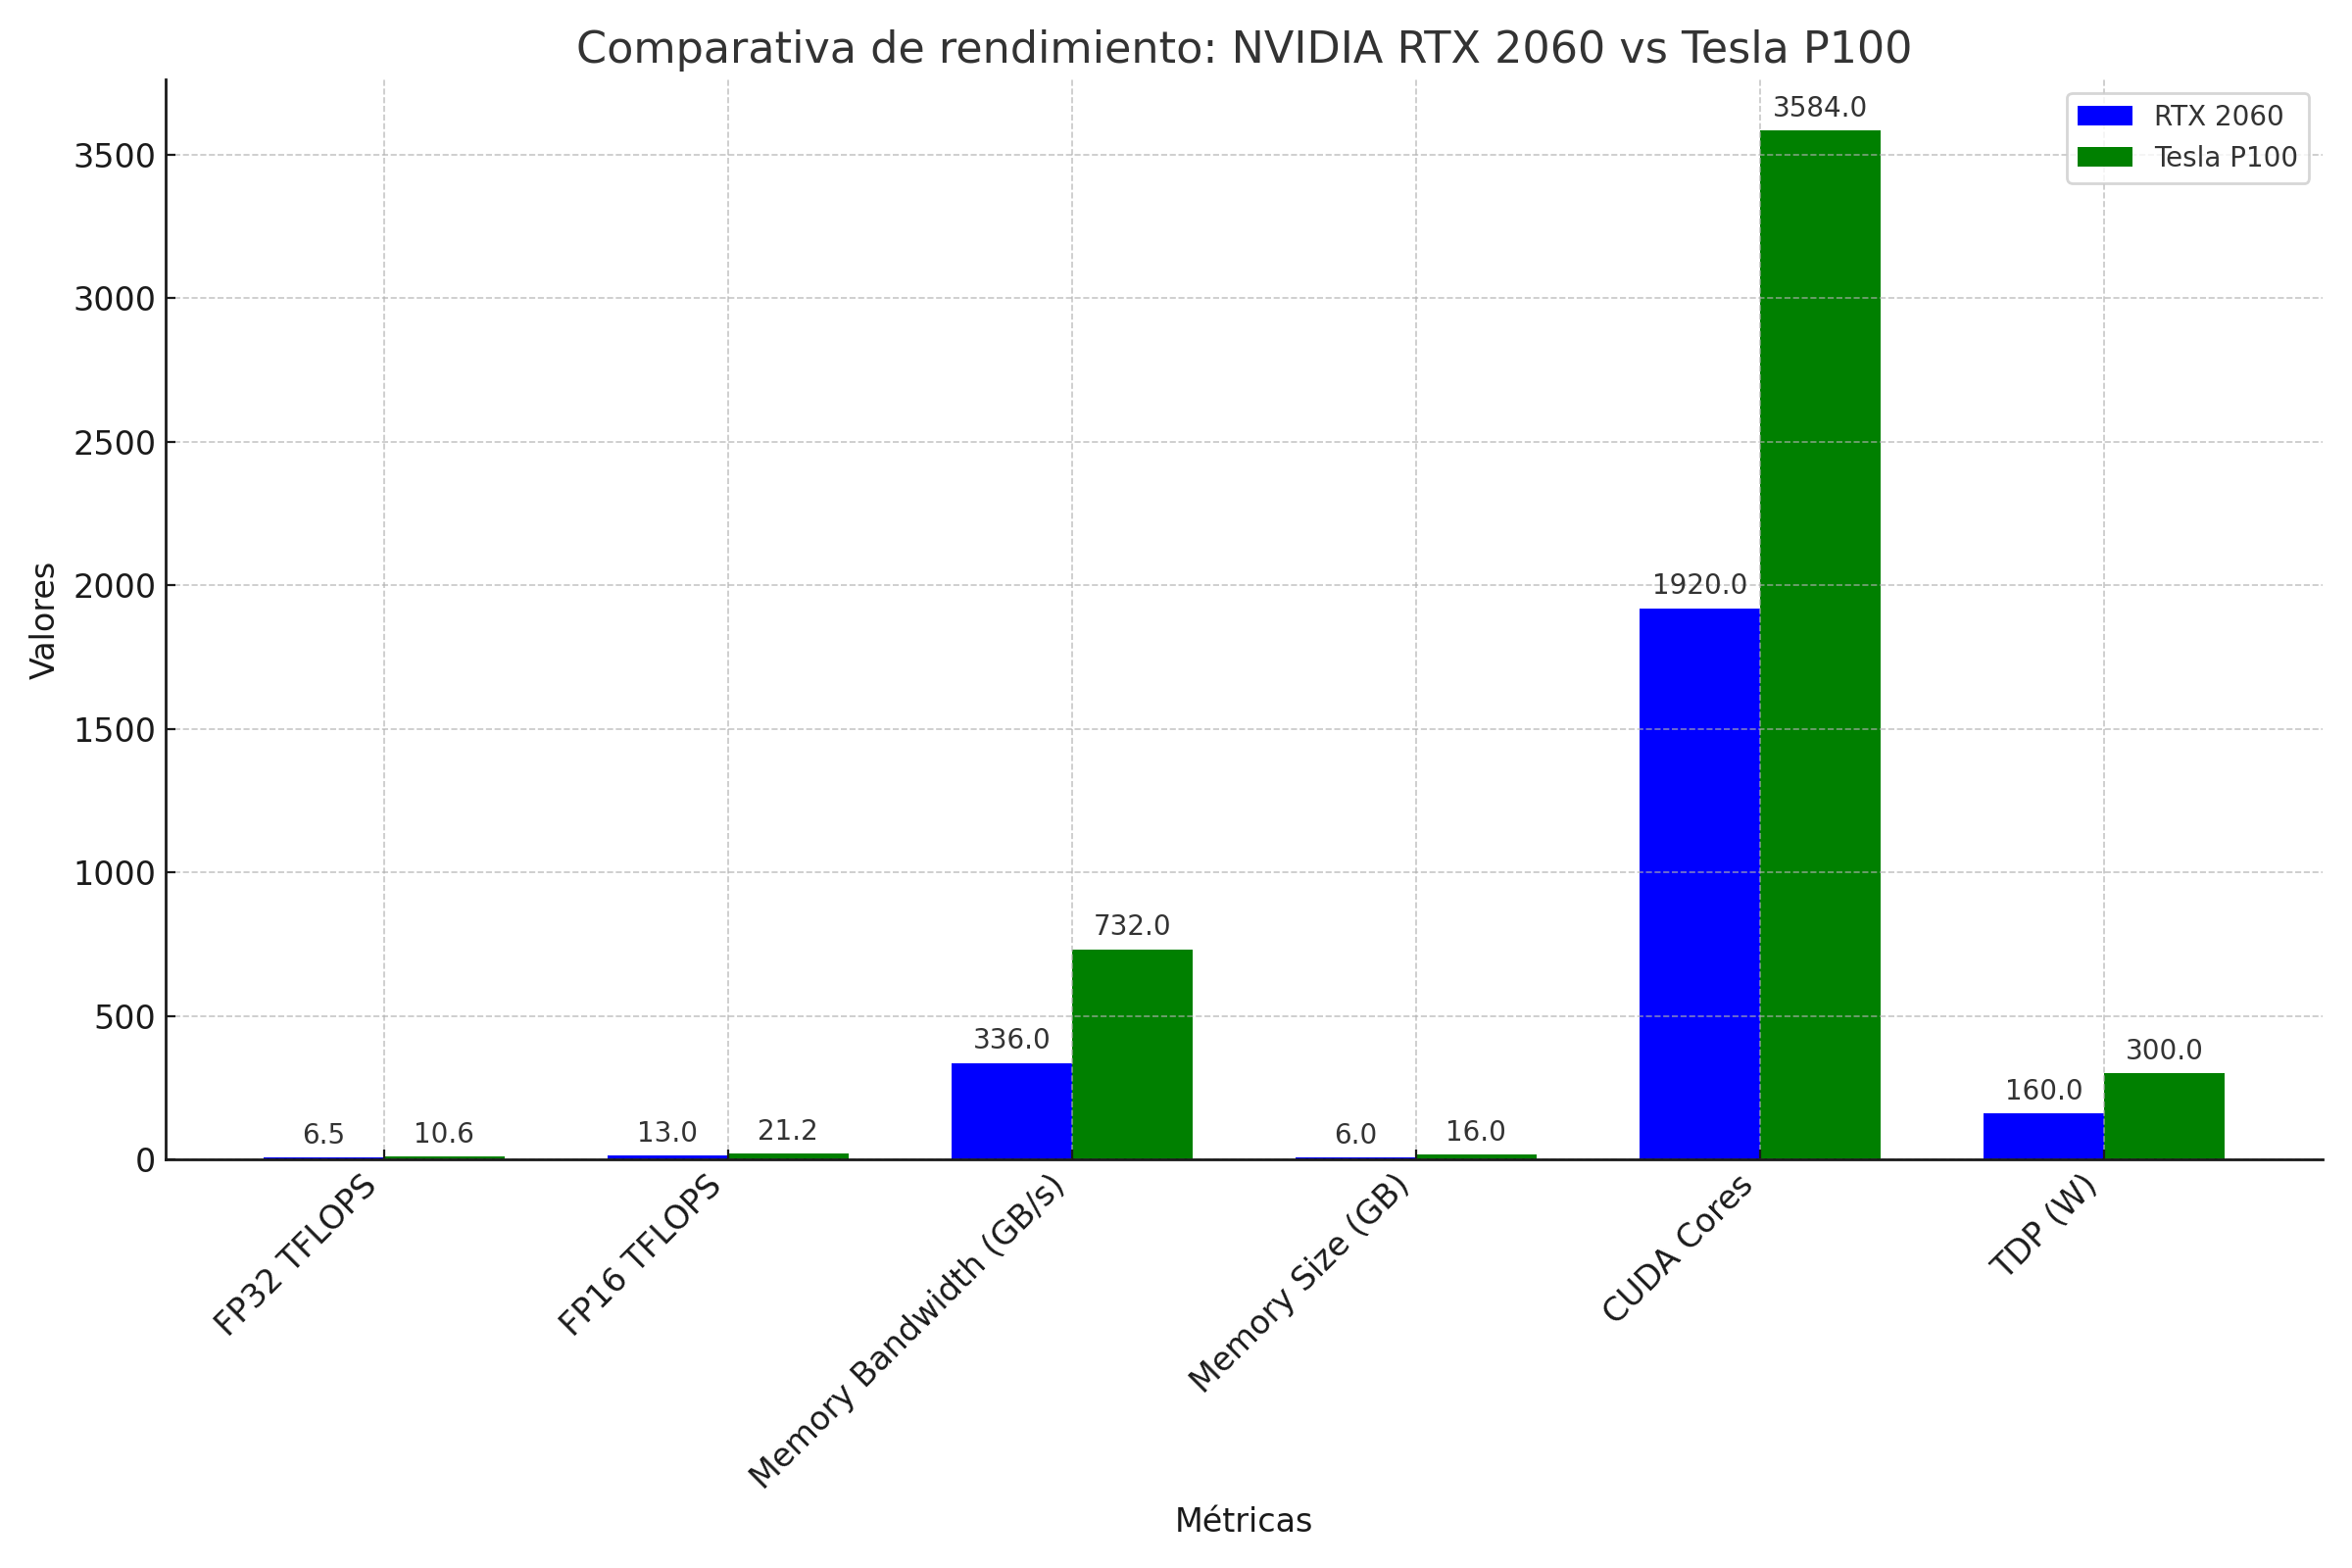
\includegraphics[width=1.0\linewidth]{imagenes/comparativa_rtx2060tesla.png}
		\caption{Comparativa de rendimiento de las GPU disponibles}
	\end{figure}
	
	En todas las características la gráfica ofrecida por Kaggle supera a la nuestra. Por lo que optaremos por usarla en todo el trabajo.
	
	\item \textbf{Hardware para inferir con los modelos}. Para la construcción de la interfaz y su uso si hemos usado nuestro dispositivo personal.
	
	De forma general, el hardware necesario para inferir con los modelos es cualquier PC de uso personal que disponga de una GPU de rendimiento similar o mejor que el nuestro y cumpla las siguientes dependencias (link a apéndice de uso del programa). 
	
\end{enumerate}


\section{Preprocesado de Datos}

En este apartado se explicará el preprocesamiento que se ha aplicado a las resonancias magnéticas para convertirlas a entradas de los modelos. 

Partiendo de nuestro conjunto de datos que presentamos en la introducción obtenido de la competición BraTS en Synapse. Ya vemos como las resonancias presentan características favorables para ser una entrada a la red.

\begin{enumerate}
	\item \textbf{Dimensiones estandarizadas} : Todas las resonancias (adultos, niños, diferente tipo de tumor) presentan las mismas dimensiones.
	\item \textbf{Imágenes estandarizadas} : Todas las resonancias se han hecho con el mismo estándar de escáner, todas presentan el mismo rango para su visualización. 
	\item \textbf{No existen valores faltantes} : Observamos como el conjunto de datos es completo en su definición, todas las resonancias de cada paciente tienen las mismas cuatro pruebas.
\end{enumerate}

\subsection{Elección de dimensionalidad de las entradas}

Una de las elecciones cruciales al inicio del trabajo es la dimensionalidad de las entradas de la red (determina la forma en la que preprocesaremos los datos). ¿Es mejor trabajar en 2D con una única imagen como entrada o en 3D con todo el conjunto de imágenes de una resonancia como entrada?

En un primer momento debido a que la mayoría de literatura actual trabaja en 3D, intentamos trabajar en 3D. Para ello, construimos un primer modelo inicial de arquitectura para 2D y  una forma de transformarlo a 3D es simplemente duplicar cada capa por la cantidad de imágenes en cada resonancia. Por lo que, el tamaño de nuestro modelo inicial 2D $SIZE_{2D}$ sólo debíamos multiplicarlo por la cantidad de imágenes en una resonancia $SIZE_{3D} = SIZE_{2D} \times 155 $. Debido que el máximo de memoria RAM que disponíamos en la Tesla P100 de Kaggle es $16\ GB$ siguiendo esa regla, el máximo tamaño que podría ocupar un modelo inicial 2D sería: 

$$ MAXSIZE_{2D} = \frac{16\ GB}{155}  = 0.10323\ GB = 105.7\ MB $$  

Esta cantidad de memoria para una arquitectura que obtenga resultados competentes en la actualidad de técnicas que existen no es viable. Viéndonos obligados ante la escasez de memoria en GPU a enfocar nuestros esfuerzos en una dimensionalidad 2D. Tendremos como entrada a las arquitecturas \textbf{una única imagen la correspondiente a la vista axial de las resonancias}.

\subsection{Normalizado de las imágenes}

Las imágenes que componen las resonancias son mapas en escala de gris donde un píxel de la imagen puede tomar un valor de gris en el intervalo $[0, 256)$. Entre las imágenes de distintas resonancias se encuentra una misma distribución de valores de píxeles para representar la misma información. Sin embargo, el proceso de entrenamiento no deja de ser un proceso de optimización y puede que este rango sea aún demasiado grande.

Adicionalmente, para evitar posibles píxeles erróneos en la toma de las imágenes que podamos interpretar como outliers que tengan un impacto negativo en el entrenamiento y para hacer las imágenes más interpretables se aplica a las imágenes normalización Z-score o estandarización.

$$ X_{std}^{i}= \frac{x^{i}-mean}{std} $$



\subsection{Recortado de imagen}

Podría ser razonable reducir las dimensiones de las imágenes para hacer a nuestros datos menos pesados. Sin embargo, se opta por no hacerlo por seguridad y escalibilidad. BraTS fija esas dimensiones en base del estándar en una resonancia magnética, así para cualquier paciente se garantiza que la imagen de su cerebro se puede representar en una resonancia en unas condiciones de resolución iguales al resto de pacientes.

Si recortamos las imágenes de forma cuadrada al cerebro más grande de todas las resonancias, podríamos encontrarnos en inferencia con un cerebro mayor que no se podría representar en una imagen. Es necesario dejar cierto margen, optando por respetar el margen inicial que marcan los organizadores médicos de BraTS.

\subsection{Undersampling}

En el estado del arte ya mencionamos que existía un desbalanceo entre tejido sano y tejido enfermo. En la mayoría de resonancias existe una mayor proporción de tejido sano que de tejido enfermo. Esto no sólo podía introducir un sesgo en los algoritmos de segmentación sino que aumenta mucho el coste computacional de entrenar a los modelos por el exceso de imágenes que no contienen la información de una lesión tumoral. 

El tratamiento del desbalanceo mediante undersampling siempre es una medida agresiva ya que podría eliminar información que a priori no consideramos relevante y si lo es.

Sin embargo, en nuestro problema aplicaremos undersampling con el principal objetivo de reducir los tiempos de entrenamiento y poder tener una arquitectura más profunda manteniendo tiempos razonables. Intentando aliviar de paso el problema del desbalanceo. A continuación explicamos en detalle como se ha llevado a cabo.

Para todo nuestro conjunto de datos $X$ creamos archivos CSV para cada partición (entrenamiento, validación y test) donde cada fila de cada archivo CSV representa a una imagen o entrada a la red. 

Estos archivos en formato CSV contendrán únicamente el conjunto de imágenes que contienen lesión tumoral de todas las resonancias $N$ más una parte seleccionada aleatoriamente de imágenes sin lesión de tamaño $\frac{|N|}{2}$. De esta forma, nos quedamos con todas las imágenes con información de lesión y con una parte representativa y balanceada sin lesión para no sesgar al modelo a segmentar en todas las imágenes.

En estos archivos CSV existen las siguientes columnas:

\begin{enumerate}
	\item \textbf{Rutas absolutas} : En $4$ columnas están las rutas absolutas a los archivos .nii de cada prueba de cada resonancia.
	\item \textbf{Número de slice} : Se guarda el número de slice en la que se localiza esa imagen dentro de la resonancia. Este campo es necesario para poder extraer la imagen.
	\item \textbf{Etiqueta} : Para el problema de clasificación es necesario guardar la etiqueta que identifica a cada imagen, 0 para Glioblastoma, 1 para Meningioma y 2 para No Tumor.
\end{enumerate}

Tras aplicar este undersampling nos quedamos con $74487$ imágenes en entrenamiento, $31899$ en validación y $45354$ en test. En la siguiente tabla podemos ver recogida esta información también términos de porcentaje respecto las imágenes totales.

\begin{table}[H]
	\centering
	\begin{tabular}{|c|c|c|c|}
		\hline
		\textbf{Partición} & \textbf{Pacientes} & \textbf{Imágenes} & \textbf{Porcentaje $\%$} \\ \hline
		Entrenamiento & 1033 & 74487 &  46.52 \\ \hline
		Validación & 442 & 31899 & 46.56 \\ \hline
		Test & 632 & 45354 &  46.3\\ \hline
	\end{tabular}
	\caption{Porcentaje de imágenes conservadas tras undersampling.}
\end{table}


\section{Elección de modelos}

A continuación pasamos a discutir los modelos y técnicas empleadas para la creación de las arquitecturas. En este trabajo como al igual que en parte del estado del arte combinaremos técnicas de aprendizaje no supervisado y supervisado.

\subsection{Codificador y representación latente}

Ponemos ahora el foco en un modelo en principio pensado para el aprendizaje sin etiquetas, los \textbf{autoencoders}.

Los autoencoders son arquitecturas encoder-decoder con la finalidad de aprender las características de un conjunto de datos o distribución. Por ejemplo, siendo esto útil para obtener modelos generativos como los autoencoders variacionales. 

Los autoencoders se formularon inicialmente como una generalización no lineal del análisis de componentes principales (PCA) por su poder para reducir la dimensionalidad. En este trabajo lo incluiremos como modelo base para aplicar aprendizaje no supervisado y que teóricamente presentarían notables ventajas de cara obtener una mayor convergencia y generalización en el proceso de entrenamiento. 

A continuación, mostramos un esquema explicativo de las partes implicadas en la arquitectura para construir el codificador y representación latente.

\begin{figure}[H]
	\centering
	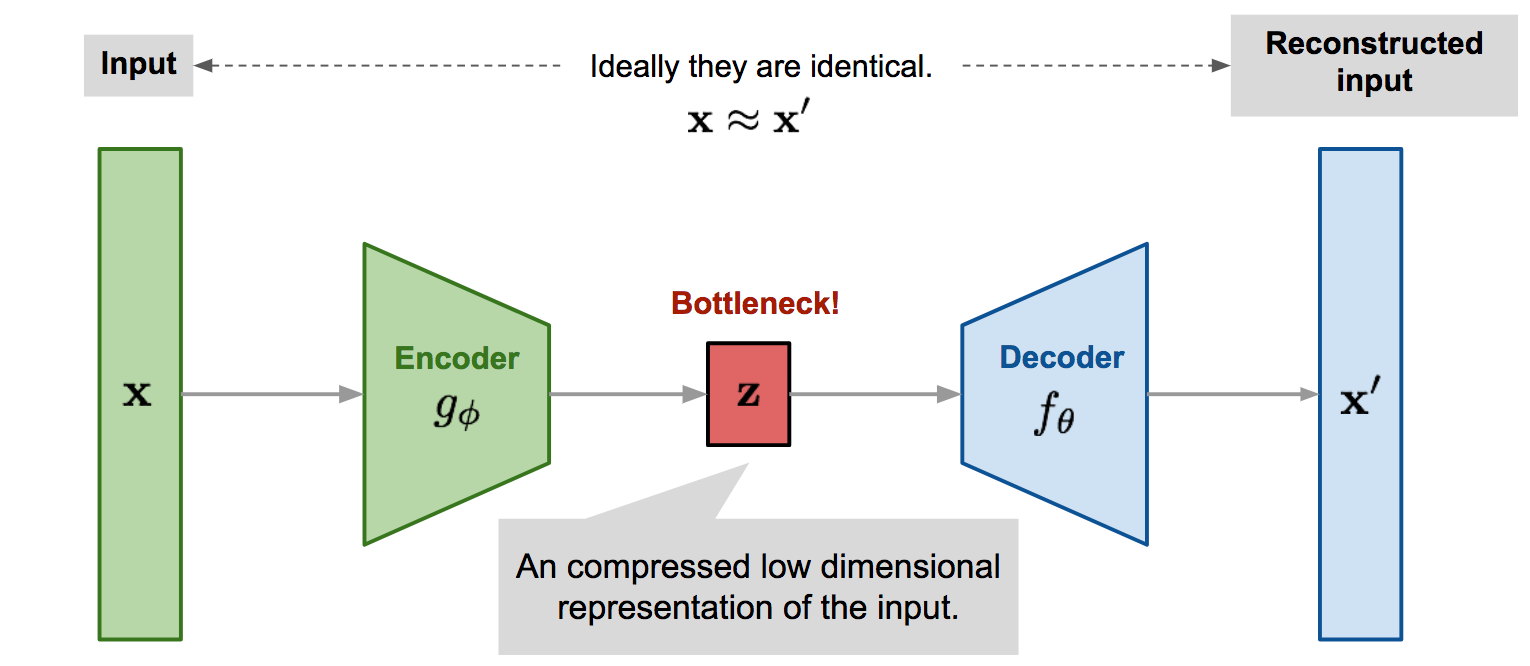
\includegraphics[width=1.0\linewidth]{imagenes/esquema_codificador.png}
	\caption{Esquema de la arquitectura empleada para inicializar el codificador y representación latente}
\end{figure}


El objetivo tras aplicar este esquema es construir un fuerte codificador que reduzca la dimensionalidad y una representación latente (bottleneck) que comprima las características principales de las imágenes del conjunto de entrenamiento.

En términos del proceso de optimización que es el entrenamiento, de forma no supervisada se están inicializando los pesos de la red para parecerse al conjunto de imágenes. \cite{zeiler2014visualizing} estudia como los diferentes filtros de las redes neuronales convolucionales al entrenarse ante una tarea de clasificación acaban replicando las características generales y específicas de las imágenes de las que son entrenados. Por ello, se llega a la conclusión de que una heurística importante dentro de las redes neuronales convolucionales es que \textbf{los filtros se parecen a las imágenes}. 

Esta razón explica de forma teórica como un proceso de ajuste previo al conjunto de entrenamiento elimina el coste computacional de búsqueda de los pesos via descenso del gradiente y backpropagation que require el ajuste de la red por sí misma a las imágenes sólo a partir de las etiquetas. 

\subsection{Uso de transfer learning}

\subsection{Modelo de clasificación}

\subsubsection{Esquema de votación}

\subsection{Modelo de segmentación}

\section{Diseño de las arquitecturas}

En el siguiente apartado detallaremos los módulos y capas que componen a las arquitecturas así como las componentes importantes. 

\subsection{Función de activación}

Para todas las arquitecturas (segmentación, clasificación y el autoencoder para construir el codificador), se optará por el uso de la función de activación ReLU (Rectified Linear Unit), definida como:

$$ \text{ReLU}(x) = \max(0, x) $$

Donde \( x \) es la entrada a la función ReLU.

A continuación, enunciamos algunas de las razones de su elección y su reconocida robustez para una gran amplitud de problemas en aprendizaje profundo.

\begin{enumerate}
	\item \textbf{No Linealidad:}
	ReLU introduce no linealidad en las redes neuronales, lo cual es crucial para que las redes puedan aprender y modelar relaciones y características complejas en los datos. Esta no linealidad es esencial para tareas como la clasificación y la segmentación, donde las relaciones entre los datos son inherentemente no lineales.
	
	\item \textbf{Gradiente Constante:}
	Para valores positivos de $ x $, la derivada de ReLU es constante e igual a 1. Esto evita el problema del desvanecimiento del gradiente en redes profundas, donde el gradiente puede volverse extremadamente pequeño en funciones de activación saturadas como la sigmoide y la tangente hiperbólica.
	
	\[ \frac{\partial \text{ReLU}(x)}{\partial x} = \begin{cases} 
		1 & \text{si } x > 0 \\
		0 & \text{si } x \leq 0 
	\end{cases} \]
	
	Esto facilita el entrenamiento de redes más profundas y la convergencia más rápida durante el proceso de optimización.
	
	\item \textbf{Eficiencia Computacional:}
	La función ReLU es eficiente en términos computacionales. Su implementación es simple (una comparación y una operación de máximo) y no involucra cálculos costosos como funciones exponenciales.
	
\end{enumerate}

La elección de ReLU como función de activación común a través de estas arquitecturas se basa en sus propiedades matemáticas que promueven la eficiencia, la no linealidad y la estabilidad del gradiente.


\subsection{Construcción del codificador y representación latente}

\subsubsection{Reducción de canales}

\subsection{Arquitectura para clasificación}

\subsection{Arquitectura para segmentación}

\section{Optimización de las arquitecturas}

En la siguiente sección detallaremos las funciones de pérdida usadas en cada arquitectura y la metodología seguida para llevar a cabo el entrenamiento de la red.

\subsection{Optimizador}

\subsection{Funciones de pérdida}

\subsubsection{Función de pérdida para la reconstrucción de imágenes}

Usamos el \textbf{error absoluto medio} (MAE) de los píxeles de salida reconstruidos y los verdaderos como función de pérdida para realizar la reconstrucción de las imágenes. El MAE mide la magnitud promedio de las diferencias absolutas entre los valores predichos por el modelo y los valores reales. Esta métrica es útil para evaluar la precisión de la reconstrucción de las imágenes, ya que considera todas las diferencias de manera uniforme, sin penalizar más las diferencias grandes que las pequeñas.

$$ \text{MAE} = \frac{1}{n} \sum_{i=1}^{n} \left| y_i - \hat{y}_i \right| $$ 

Donde $n$ es el número total de píxeles en la imagen, $y_i$ es el valor verdadero del píxel $i$ y $\hat{y}_i$ es el valor reconstruido o predicho del píxel $i$.

En el contexto de la reconstrucción de imágenes, cada $y_i$ representa la intensidad del píxel en la imagen original, y cada $\hat{y}_i$ representa la intensidad del píxel en la imagen reconstruida por el modelo. El MAE proporciona una medida directa de cuán cerca están las intensidades de los píxeles reconstruidos de las intensidades reales.

También usaremos la misma pérdida como métrica de bondad de ajuste del modelo. Esto significa que, además de utilizar el MAE para optimizar el modelo durante el entrenamiento, también lo emplearemos para evaluar el desempeño del modelo en la reconstrucción de imágenes. Utilizar el MAE como métrica de evaluación nos permite tener una interpretación clara y consistente de cómo de bien se está desempeñando el modelo en términos de error promedio de los píxeles reconstruidos.

\subsubsection{Función de pérdida para clasificación}

Focal Loss es una función de pérdida que se ha demostrado ser particularmente efectiva para problemas de clasificación, especialmente en contextos donde hay un desequilibrio en las clases o cuando algunas muestras son más difíciles de clasificar que otras. Tras el procesamiento de datos, no existe un desbalanceo de datos grande. Sin embargo, la naturaleza de los tumores hacen que existan imágenes muy variables entre sí (con distinto grado de dificultad de optimización) es por ello que se opta por una pérdida que tenga algún mecanismo de control sobre esto. A continuación se explica por qué la Focal Loss puede ser mejor que la tradicional Cross Entropy Loss, especialmente en el contexto de datos con diferentes niveles de dificultad:

La Cross Entropy Loss es la función de pérdida estándar para problemas de clasificación y se define como:
$$  {\text{CE}} = - y_i \log(p_i) $$
$$  L_{\text{CE}} = - \sum_{i=1}^N y_i \log(p_i) $$

donde $y_i$ es la etiqueta verdadera y $p_i$ es la probabilidad predicha de la clase correcta. Aunque es efectiva, tiene algunas limitaciones:
\begin{enumerate}
	\item \textbf{Tratamiento Igualitario de todos los ejemplos}: Cross Entropy Loss trata todos los ejemplos de entrenamiento por igual, sin importar si son fáciles o difíciles de clasificar.
	\item \textbf{Sensibilidad al desbalanceo de clases}: No maneja bien los datos desbalanceados, donde algunas clases son mucho más frecuentes que otras.
\end{enumerate}

Focal Loss, propuesta por \cite{lin2017focal}, introduce un término adicional para enfocar el entrenamiento en ejemplos más difíciles. Se define como:

$$ {\text{FL}} = - \alpha (1 - p_t)^\gamma \log(p_t) $$
$$ L_{\text{FL}} = - \sum_{i=1}^N \alpha_t (1 - p_{t_i})^\gamma \log(p_{t_i})$$

donde $p_t$ es la probabilidad predicha de la clase correcta, $\alpha$ es un factor de ponderación para balancear la importancia de las clases, y $\gamma$ es el parámetro de focalización. Se puede desarrollar su principal ventaja:

\begin{enumerate}
	\item \textbf{Enfoque en ejemplos difíciles}: El término $(1 - p_t)^\gamma$ reduce la pérdida para los ejemplos bien clasificados (donde $p_t$ es alto) y mantiene alta la pérdida para los ejemplos mal clasificados (donde $p_t$ es bajo).
	
	\begin{enumerate}
		\item Cuando un ejemplo es fácil de clasificar ($p_t$ es alto), el término $(1 - p_t)^\gamma$ es pequeño, reduciendo su contribución a la pérdida total.
		\item Cuando un ejemplo es difícil de clasificar ($p_t$ es bajo), el término $(1 - p_t)^\gamma$ es grande, incrementando su contribución a la pérdida total.
	\end{enumerate}
	
	\item \textbf{Parámetro de Focalización}: El parámetro $\gamma$ ajusta el grado de focalización. Con $\gamma=0$, Focal Loss se reduce a la Cross Entropy Loss. Valores más altos de $\gamma$ incrementan el enfoque en los ejemplos difíciles.
	
	\item \textbf{Reducción del impacto de ejemplos fáciles}: Dado que los ejemplos fáciles no dominan el gradiente debido al término de focalización, el modelo no se sesga hacia las clases dominantes o los ejemplos que ya son bien clasificados.
	
\end{enumerate}

Esto implica los siguientes beneficios cuando existen datos de diferente dificultad.

\begin{enumerate}
	\item \textbf{Mejora del rendimiento general}: En muchos problemas de clasificación, hay ejemplos que son intrínsecamente difíciles de clasificar debido a la superposición de clases, ruido en los datos, o características ambiguas. Focal Loss ayuda a mejorar el rendimiento general del modelo al hacer que el modelo preste más atención a estos ejemplos difíciles durante el entrenamiento.
	
	\item \textbf{Mejor manejo de outliers}: Al reducir la contribución de ejemplos fáciles a la pérdida total, Focal Loss puede ayudar a mitigar el impacto de outliers o ejemplos atípicos que podrían desviar el modelo cuando se usa Cross Entropy Loss.
	
	\item \textbf{Robustez en modelos de gran escala}: En problemas similares como la detección de objetos en imágenes, donde el desequilibrio entre fondo y objeto puede ser significativo y algunos objetos son más difíciles de detectar que otros, Focal Loss ha demostrado ser particularmente útil.
	
\end{enumerate}

Focal Loss es una mejora sobre Cross Entropy Loss al proporcionar un mecanismo para enfocarse en ejemplos díficiles tales como imágenes donde los tumores sean pequeños. Con la gran en este problema de que realmente no queremos principalmente predecir muy bien la mayoría de ejemplos sino ser precisos en los ejemplos especialmente difíciles también para el personal médico. Por todo ello, se opta por utilizar \text{Focal Loss} para la primera tarea de clasificación.

\subsubsection{Función de pérdida para segmentación}

Como función de pérdida en segmentación se escoge el complemento negativo de su métrica más importante \textbf{similaridad Dice}: \textbf{Dice Loss}. Dice Loss se define como:

$$ L_{dice} = 1 - Dice(A, B) $$

Por lo tanto,  \textbf{Dice Loss} varía entre 0 y 1, donde 0 indica una superposición perfecta y 1 indica ninguna superposición (es decir, pérdida máxima).

Podemos enumerar las características que hacen de Dice Loss una de las pérdida más acertadas para la segmentación de tumores cerebrales. 

\begin{enumerate}
	\item \textbf{Sensibilidad a pequeñas áreas}: En la segmentación de tumores cerebrales, es crucial detectar incluso pequeñas regiones de tumores. El Dice Loss está diseñado para ser sensible a estas pequeñas áreas de superposición, lo que permite que el modelo se entrene para identificar y segmentar con precisión los bordes y áreas menos visibles del tumor.
	
	\item \textbf{Interpretabilidad clínica directa}: El coeficiente de similaridad Dice, en el que se basa el Dice Loss, proporciona una medida directa de cuán bien la predicción del modelo coincide con la realidad clínica. Esta métrica es intuitiva para los profesionales de la salud, ya que refleja la precisión de la segmentación en términos de superposición de áreas tumorales detectadas.
	
	\item \textbf{Robustez ante desbalanceo en la distribución de clases}: Los tumores cerebrales pueden representar solo una pequeña fracción de la imagen total, lo que genera desequilibrios en la distribución de clases. Dice Loss maneja este desequilibrio al penalizar menos la falta de predicción en áreas dominadas por el tejido cerebral normal, centrándose en mejorar la detección precisa de los tumores.
	
	\item \textbf{Optimización efectiva en el entrenamiento}: El uso de Dice Loss proporciona una superficie de optimización más suave y estable durante el entrenamiento de modelos de segmentación que otras pérdidas. Esto facilita la convergencia del modelo y reduce la necesidad de ajustes complejos de hiperparámetros, mejorando así la eficiencia del entrenamiento y la calidad de las segmentaciones obtenidas.
\end{enumerate}


\subsection{One-Cycle Policy}

La \textbf{política 1cycle} fue propuesta por \cite{smith2019super}, y es una técnica de programación de tasas de aprendizaje para mejorar el rendimiento del entrenamiento de redes neuronales. El objetivo principal es encontrar tasas de aprendizaje que aceleren el entrenamiento y mejoren la generalización del modelo. También ajusta la tasa de aprendizaje durante el entrenamiento de manera específica en función del número de iteraciones. Esta utiliza un ciclo de entrenamiento único en lugar de tasas de aprendizaje fijas durante todo el entrenamiento. Durante este ciclo, la tasa de aprendizaje varía de manera cíclica desde un valor inicial hasta un valor máximo y luego vuelve a descender.

En la primera mitad del ciclo, la tasa de aprendizaje aumenta gradualmente desde un valor inicial hasta un valor máximo. Este aumento permite una exploración más rápida del espacio de parámetros y puede ayudar a escapar de mínimos locales subóptimos. En la segunda mitad del ciclo, la tasa de aprendizaje disminuye gradualmente desde el valor máximo hasta el valor inicial. Esto permite una refinación más precisa de los pesos del modelo y una convergencia más estable hacia el mínimo global.

Además de ajustar la tasa de aprendizaje, la política 1cycle también propone variar el \textbf{momentum} (una técnica que ayuda a acelerar el entrenamiento). El momentum se incrementa en la fase de aumento y disminuye en la fase de descenso.

La política 1cycle también actúa como una forma de regularización. El uso de tasas de aprendizaje más altas en la fase de aumento y más bajas en la fase de descenso puede ayudar a prevenir el sobreajuste. También sugiere seleccionar los valores iniciales y máximos de la tasa de aprendizaje de manera específica. El valor máximo de la tasa de aprendizaje se elige típicamente como un valor que es varias veces mayor que el valor inicial.

La duración total del ciclo puede variar, pero en general, se sugiere que sea aproximadamente igual al número total de épocas de entrenamiento.
La \textbf{política 1cycle} ha demostrado ser efectiva en mejorar la convergencia y la generalización en una variedad de tareas y arquitecturas de redes neuronales. Sin embargo, la selección precisa de los parámetros, como las tasas de aprendizaje inicial y máxima requiere ajustes específicos para cada objetivo y conjunto de datos.

En este trabajo usaremos esta política como forma de regularización y como método general para evitar la búsqueda de hiperparámetros manual para el proceso de aprendizaje. Para ello, en todo el trabajo sólo usaremos las llamadas a las funciones \texttt{fit\_one\_cycle()} para entrenar toda las capas de la red y \texttt{fine\_tune()} para cuando necesitemos diferenciar qué épocas entrenar toda la red (incluyendo la parte convolucional) o solo la parte densamente conectada. Ambas funciones de \textbf{Fastai} que implementan la política 1cycle. 

\section{Métricas y validación}

\section{Desarrollo para la predicción de la evolución}